\section{Strømforsyning} \label{sec:PsuImpl}

\begin{figure}[h]
\centering 
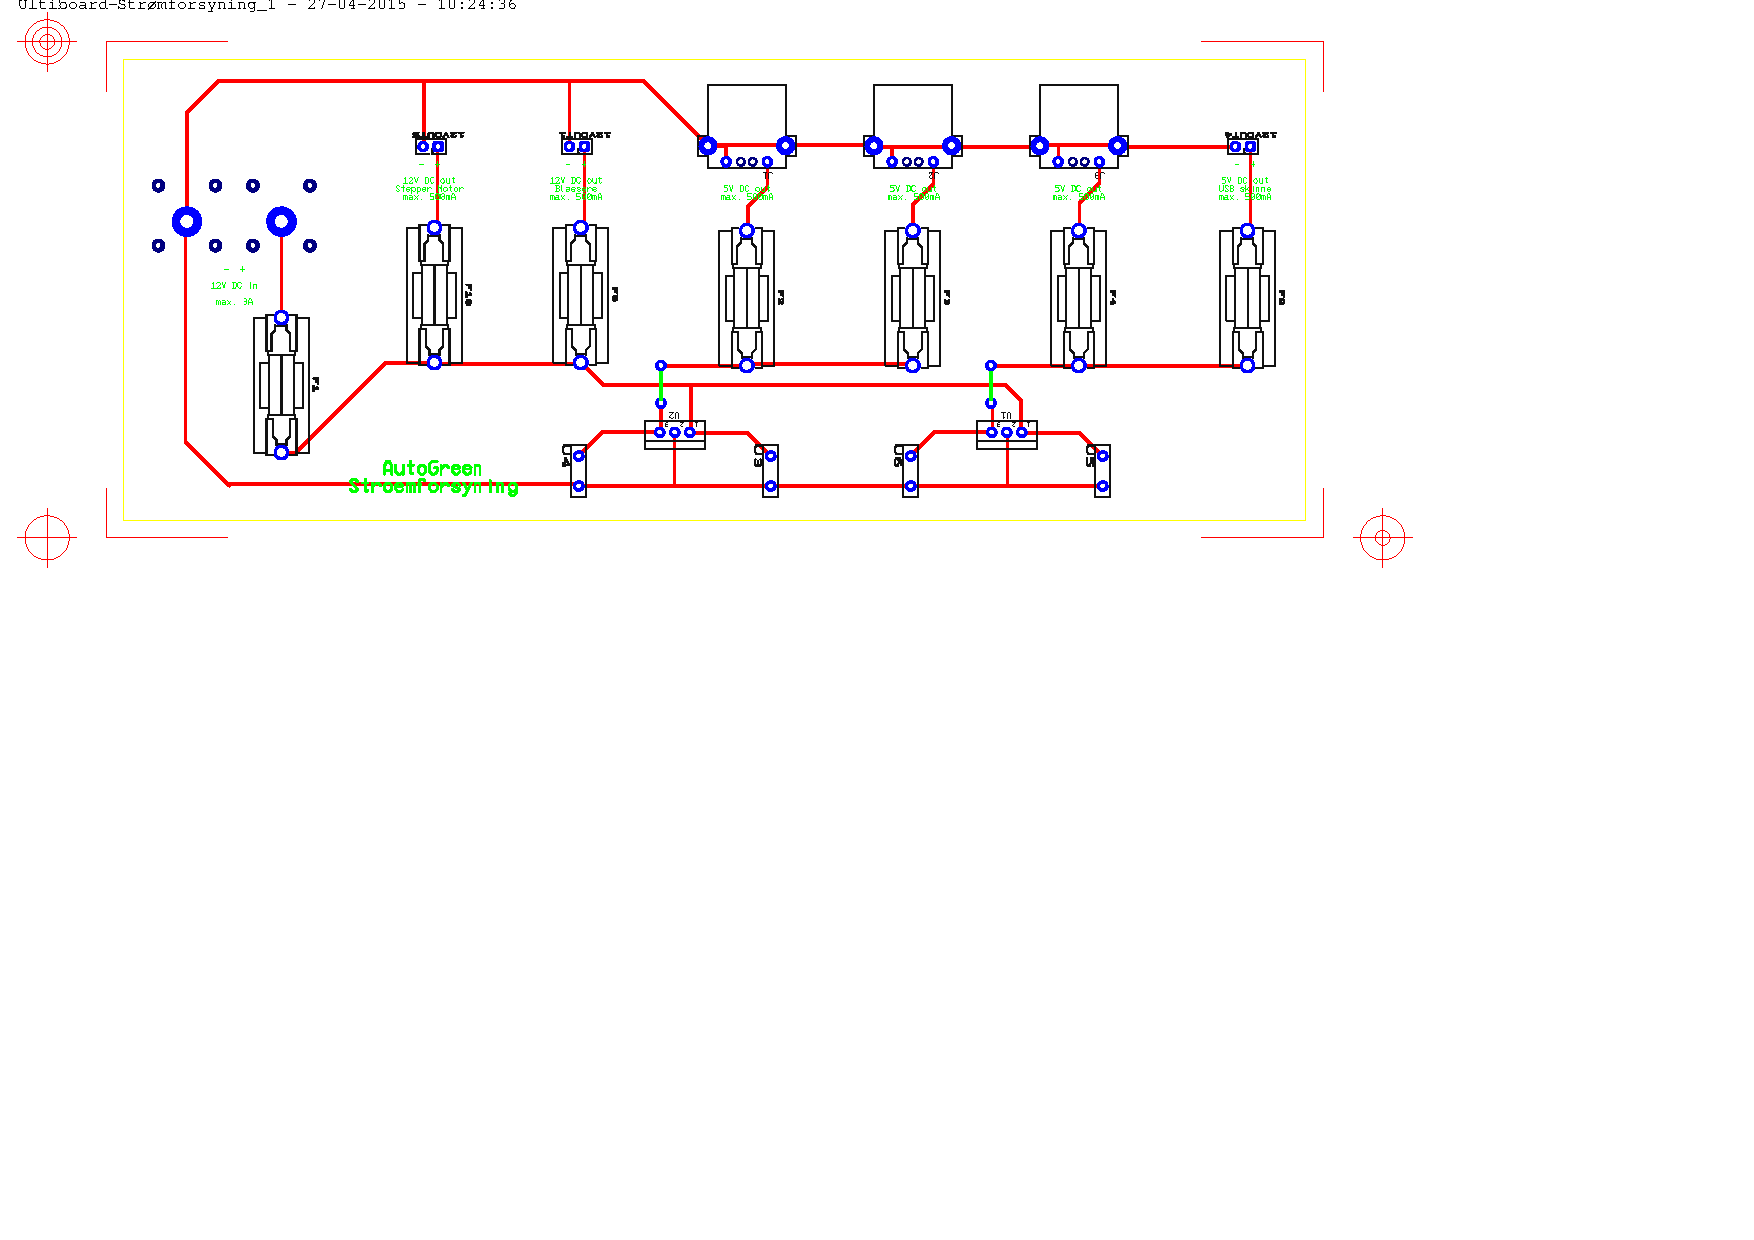
\includegraphics[width={\textwidth+2.9cm}, trim=55 345 210 25, clip=true, angle =90] {../fig/ultiboard_stroemforsyning.pdf}
\caption{Printudlæg for Strømforsyning i Ultiboard}
\label{fig:ultiboard_stroemforsyning}
\end{figure}

\clearpage

Implementering af strømforsyning foretages ved at Multisim diagrammet eksporteres til Ultiboard, hvorefter printet udlægges.
Det forsøges gjort således at printet er overskueligt, og med så få lus som overhovedet muligt. 
Som udgangspunkt er alle forbindelser på printet lagt på bagsiden. 
Det designede print er vist på Figur \ref{fig:ultiboard_stroemforsyning}. 

Kobber på undersiden af printet er vist med rød, mens kobber på oversiden af printet er vist med grøn. 
Kobberøer er vist med blå.
Der er en lille hage ved kobberøerne; der er ikke forbindelse mellem oversiden og undersiden. 
Derfor må man lodde et lille stykke monteringstråd igennem printet for at skabe forbindelse de stder hvor det er nødvendigt. 

Omkredserne af komponenterne (sort) printes ikke, de vises kun som en slags hjælpelag. 

Databasen i Ultiboard indeholder ikke komponenter til bananbøsninger, derfor er disse omkredse ikke med på figuren. 

Der skrives lidt forklarende tekst på oversiden af printet, så man kan se hvad der skal kobles til hvor; dette er lidt svært at se på figuren.
\newline

Printudlægget bestilles ved E-LAB på IHA, hvorefter komponenter loddes på.
Det færdige print er vist på Figur \ref{fig:stroemforsyning_print}.

\begin{figure}[h]
\centering 
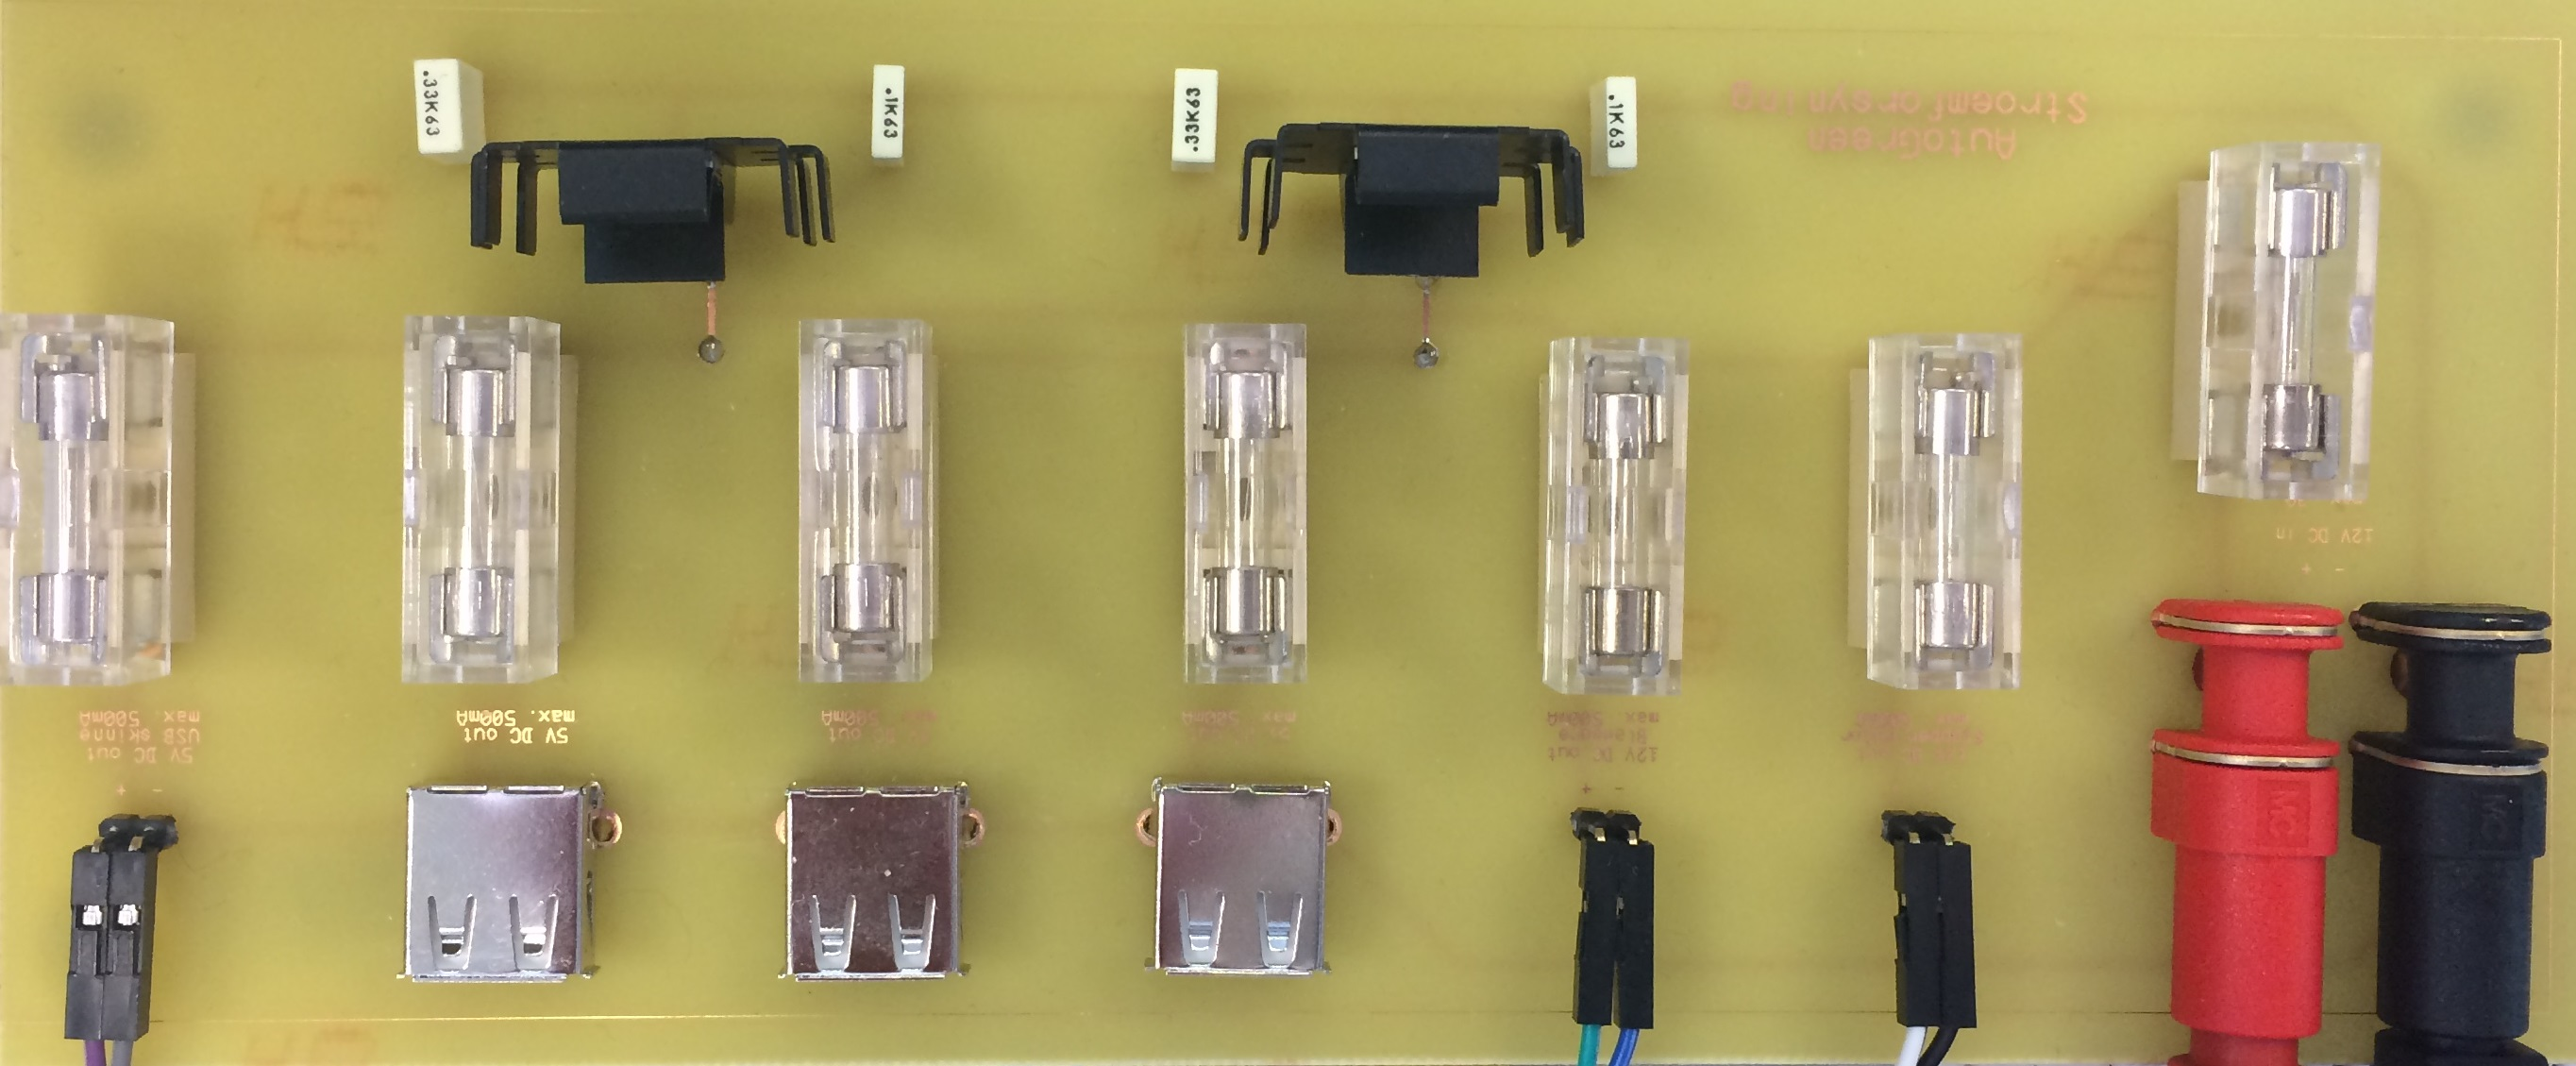
\includegraphics[width={\textwidth}, trim=0 0 0 0, clip=true] {../fig/StroemforsyningPrintBillede}
\caption{Den færdige Strømforsyning}
\label{fig:stroemforsyning_print}
\end{figure} 

\clearpage
